
\documentclass[11pt]{article}
\usepackage{amssymb}
\usepackage{graphicx}
\usepackage{amsthm}
\setlength{\textheight}{9in} \setlength{\headheight}{.2in}
\setlength{\headsep}{0in} \setlength{\topmargin}{0in}


\newtheorem{thm}{Theorem}[section]
\newtheorem{lemma}[thm]{Lemma}
\newtheorem{definition}[thm]{Definition}

\let\olddefinition\definition
\renewcommand{\definition}{\olddefinition\normalfont}

\let\olddefinition\thm
\renewcommand{\thm}{\olddefinition\normalfont}

\begin{document}
\begin{center}
Graph Masking
\end{center}
\vspace{.1in}
%\vspace{.2in}

Abstract (Kinda bad. fix later)\\
\noindent Given a graph $G(V,E)$ and a natural number $k$, we define the $k-Neighborhood$  graph of G to be $G_k(V, E_k)$, where the edge $(u,v)$ is in $E_k$ if and only if there is a path $(u,v)$ of length less than or equal to $k$ in $G$. We would like to find a $masking$ of $G$, $G'$, such that $G$ and $G'$ share a $K-neighborhood$, but no edges in $G$ can be determined by studying $G'$ ($G'$ is sufficiently random). This paper provides two heuristic algorithms to solve this problem. The first modifies $G$ to get a new graph which is guaranteed to share a $k-Neighborhood$ with $G$, but may not be sufficiently random. The second algorithm builds the new graph by continuously adding edges to an originally empty graph. The new graph is sufficiently random from the original graph, but may not share the same $k-Neighborhood$.
\\\\

%write introduction

\section{Introduction}

\subsection{Motivation}

\noindent Social networks provide means to create and maintain meaningful connections between people. They foster environments where people can not only connect with people with whom they have a previous relationship, but with entirely new people as well; without a proper way to introduce people to others with whom they may have relevant connections, there is little room for social networks to grow and provide anything worthwile to their users. \\

\noindent As social networks, such as LinkedIn, hold all the data on connections between their users, they too hold the tools to make suggestions to users on which people to seek out for connections; however, this information must be used carefully. Users put their trust in the social networks that their private information will be kept safe and not disclosed to anyone else, so security is a major factor to be considered while trying to implement methods to expand the network.  \\

\noindent In order to give the users relevant suggestions to expand their personal connections, a subset of the information held by the networks must be given such that it both is helpful to the users and does not infringe on the  privacy of others. \\

\subsection{Approach}

\noindent This paper describes a method that looks at the connections between users to determine useful information to make available to a given user so that he/she may gain new meaningful connections. This includes a label-swapping algorithm and an edge adding algorithm. Algorithms were also designed to try to test the difficulty of accurately extracting any private information from the information given. All algorithms were evaluated for computational efficiency and data was taken to evaluate them overall.  \\

\section{Basic Definitions and Notation}

\begin{definition}
A \emph{graph} is a 2-tuple $G = (V,E)$, where $V = \{v_1,v_2,...,v_n\}$ is a set of vertices (nodes) and the set of edges is $E = \{e_1,e_2,...,e_m\} \subseteq V \times V$. All edges in $E$ are undirected. Unless otherwise stated, when discussing a graph $G=(V,E)$, $v,u,w \in V$ and $e \in E$. 
\end{definition}

\begin{definition}
 A \emph{path} $P$ of length $l$ in $G$ is a sequence of edges in $E$ of the form $e_1', e_2', ...,e_l'$ such that $e_i' = (v,u)$ and $e_{i+1}' = (u,w)$ for all $i \in [1,l]$. If $e_1' = (v_0', v1')$ and $e_l' = (v_{l-1}', v_l')$, then $P$ is a path from $v_0'$ to $v_l'$. 
\end{definition}

\begin{definition}
Let $k$ be a positive integer. The \emph{k-neighborhood} of a node $v \in V$ in a graph $G = (V,E)$, denoted $N_k(v)$ is the set of all $u \in V$ where there exists a path from $v$ to $u$ of length less than or equal to $k$. The k-neighborhood of $G$ is the graph $N_k(G) = (V, E')$ where $(u,v) \in E'$ iff $v \in N_k(u)$. If $N_k(G) = G'$, we say that $G$ \emph{satisfies} $G'$. 
\end{definition}

\begin{definition}
A \emph{masking} of a graph $G$ is a graph $G'$ which satisfies $N_k(G)$.\\
\end{definition}

\noindent We say that $G'$ is $\emph{sufficiently random}$ for values $\epsilon \in [0, 0.5 ]$ and $\delta \in [0,1]$ if ...



\begin{definition}
For an integer $k$ and graph $G$, we define the \emph{adjacency group} of a node $v \in V$ as the set of all $u \in V$ such that $N_k(v) = N_k(u)$. We can see that adjacency groups are equivalence classes. {\bf ADJACENCY GROUP IS ALSO DEFINED BELOW}
\end{definition}

\section{Label-Swapping Algorithm}
\indent In this section, we present the \emph{label-swapping} algorithm which takes a graph $G$ and yields $G'$, a masking of $G$.

\noindent This algorithm works by altering the original graph while maintaining the same $k-Neighborhood$. This is accomplished by partitioning the vertices of the $V$ into so-called $adjacency$-$groups$.  We define an adjacency-group, $A$, to be a maximal set of vertices in $G_k$ such that for any two vertices $a$, $b$ in $A$, $(a, b) \in E_k$, and $(a, c) \in E_k$  if and only if $(b, c) \in E_k$, where $c$ is an arbitrary vertex distinct from $a$ and $b$. By maximal, we mean that every vertex that could be in $A$ is in $A$. Every vertex in $G_k$ must be in at least one adjacency-group, even if that group is a singleton. Also, note that any vertex can be in at most one adjacency-group. If there were a vertex $a$ in two adjacency groups $A$ and $B$, then any $b \in A$ and $c \in B$ must necessarily be in an adjacency group and the maximal adjacency-group containing $A$ would be $A \bigcup B$. Therefore, the set of maximal adjacency-groups over $G_k$ forms a partition of $V$ both in the orginal graph and the k-Neighborhood graph. 

%describe finding adjacency groups?

\indent Define a $swapping$ on the adjacency-group $A$ to be a bijection from $A$ onto itself, where each vertex is mapped to a randomly chosen vertex in $A$. We can apply a swapping to every adjacency-group in $V$ so that each node, $a$, in $V$ is renamed as $swapping(a)$. More formally, if $(u,v)$ is an edge in some graph $G$, $x=swapping(u)$, and $y=swapping(v)$, then $(x,y)$ is in the graph formed by applying the swapping to $G$. See Figure 1 for an example of such a swapping.\\

\indent The label-swapping algorithms works by finding all maximal adjacency-groups and applying a random swapping to each one. The new graph formed by applying these swappings must have the same k-Neighborhood as the original graph (see Theorem 1); however, it may be possible to determine edges in the original graph from the new graph.
\\

\begin{figure}[htb]
\centering
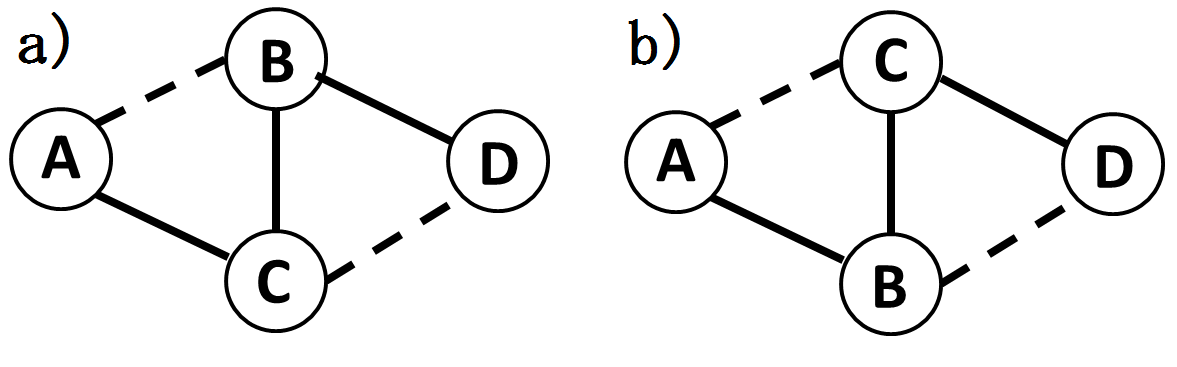
\includegraphics[scale=0.3 ]{Sample-Graph.png}
\caption{In the above graphs, solid lines represent edges in the original graph and dotted lines represent edges that are only in the 2-Neighborhood graph (Note that all edges in the original graph are necessarily in the 2-Neighborhood graph). a)  The vertices B and C are in the same adjacency-group, while A and D are each in adjacency-groups of size 1. b) The result of applying a swapping to the adjacency group containing B and C, with the 2-Neighborhood graph remaining the same as the graph in (a).}
\label{fig:sample graph}
\end{figure}


\begin{thm}  \emph{Applying a swapping to a graph, G, will yield a graph, G', with the same k-Neighborhood graph as G.}\\
\noindent \emph{Proof.} Let $G_k'$ be the k-Neighborhood graph of $G'$ and $G_k$ be the k-Neighborhood graph of $G$. Assume $G_k'$ is not equal to $G_k$. Then (i) $G_k'$ contains an edge not in $G_k$ or (ii) $G_k$ contains an edge not in $G_k'$.  \\
\indent i) Let $(u,v)$ be an edge in $G_k'$ that's not in $G_k$. Since $G'$ was formed by $swappings$ on $G$, $u$ must have some label $x$ and $v$ must have some label $y$ in $G$, where $x$ and $y$ were in the adjacency-groups of $u$ and $v$, respectively, and $(x,y)$ is in $G_k$. But, since $u$ and $x$ are in the same adjacency-group, and $(x,y)$ is in $G_k$, then $(u,y)$ must be in $G_k$. Since $y$ and $v$ are in the same adjacecy-group and $(u,y)$ is in $G_k$, then $(u,v)$ is in $G_k$, and our assumption that $G_k'$ has an edge that is not in $G_k$ must be false.\\
\indent 			ii) Let $(u,v)$ be an edge in $G_k$ that is not in $G_k'.$ Let the nodes labeled $x$ and $y$ in $G$ be given the labels $u$ and $v$, respectively, in $G'$. Therefore, $u$ and $x$ share an adjacency-group, as do $v$ and $y$.  Since $(u,v)$ is in $G_k$ and $u$ and $x$ share an adjacency-group, then $(x,v)$ is in $G_k$. Likewise, since $v$ and $y$ share an adjacency-group and $(x,v)$ is in $G_k$, then $(x,y)$ is in $G_k$. This implies that $(u,v)$ must be in $G_k'$. Therefore, our assumption that $G_k$ has an edge that is not in $G_k'$ is false. \\
By proving (i) and (ii) to be false, we can conclude that our original assumption that $G_k$ is not equal to $G_k'$ is false.\\
\end{thm}

 Edge-Adding Algorithm\\
This 

\begin{figure}[htb]
\centering
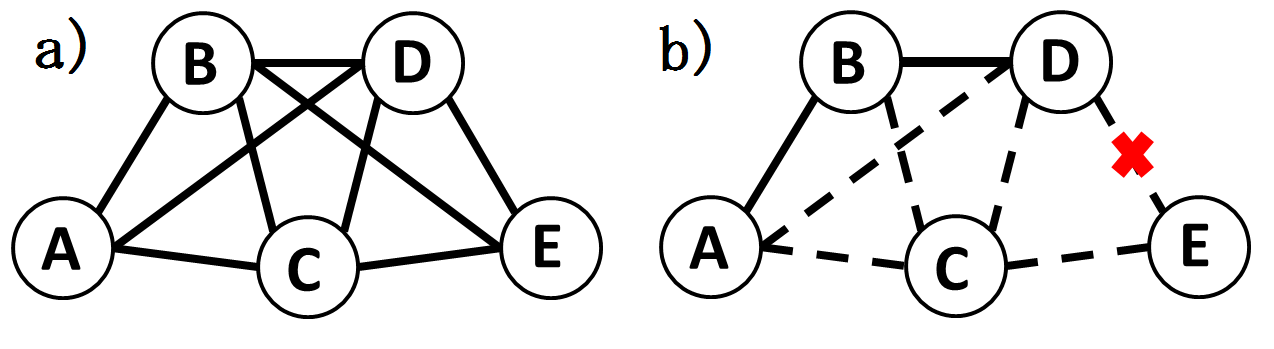
\includegraphics[scale=0.3 ]{profs_example.png}
\caption{An example of the edge-adding algorithm. a) The 3-neighborhood graph for a given input. Each edge in this graph is added to the potential-edge list at the start of the algorithm. b) The solid lines represent edges that will be in the graph the algorithm returns (edge (B,D) was the last edge added). The dotted lines are remaining edges in the potential-edge list. After (B,D) was added, there became a 2-path between A and D. Since E is not adjacent to A in the 3-neighborhood graph, the edge (D,E) was removed from the potential-edge list.}
\label{fig:profs example}
\end{figure}

\end{document}
